\documentclass[11pt]{article}
\usepackage{geometry}                % See geometry.pdf to learn the layout options. There are lots.
\geometry{letterpaper}                   % ... or a4paper or a5paper or ... 
%\geometry{landscape}                % Activate for for rotated page geometry
%\usepackage[parfill]{parskip}    % Activate to begin paragraphs with an empty line rather than an indent
\usepackage{graphicx}
\usepackage{amssymb}
\usepackage{epstopdf}
\usepackage{listings}
\usepackage{algorithm,algorithmic}
\DeclareGraphicsRule{.tif}{png}{.png}{`convert #1 `dirname #1`/`basename #1 .tif`.png}

\title{Semantic Action Notes}
\author{Dan Beatty}
%\date{}                                           % Activate to display a given date or no date

\begin{document}
\maketitle
%\section{}
%\subsection{}


Semantic Actions are embedded with the syntax analysis functions capturing the semantics of the program.. As syntax is being analyzed, a semantic representation of the program is produced.    There is such a thing as a quad table, and this table captures the meaning of the program in a concise way. 



Semantic actions are associated with the syntax production rules they accompany.    Semantics are an intricate part of a languages constructs.    Furthermore, some semantics can define the very paradigm that a language represents.  

The main semantic types shared in common with most languages are:
\begin{enumerate}
\item Expression statements
\item Conditional statements
\item Flow Control Statements
\item Declaration types
\begin{enumerate}
\item Identifier 
\item Identifier Lists
\item Array Sub lists (indices).  
\end{enumerate}
\end{enumerate}

%For instruction purposes, arrays

%\chapter {Intermediate Code Gen - Semantic Actions }

Two benefits of using intermediate - machine independent form:
\begin{quote}
\begin{enumerate}
\item Retargeting is facilitated; a compiler for a different machine can be created by attaching a back end for the new machine to an existing front end. 
\item A machine-independent  code optimizer can be applied to the intermediate representation.  
\end{enumerate}
 \end {quote} \cite{ullmanCompiler} page 463
 
 Sections 5.2 and Chapter 8 of Ullman's book deal with semantic representation.  There is a concept of three-address code from common programming language constructs.  Question, is this the same as what Cooke is calling the quads?  
 
 
 \begin{quote}
 Three address code is a linearized representation of a syntax tree or a dag in which explicit names correspond to the interior nodes of the graph.  The syntax tree and dag in Figure \ref{copy8-2} are represented by the three-address code sequences  in Figure \cite{copy8-5}.  Variable names can appear directly in three-address statements, so Figure \ref{copy8-5} (a)  has no statements corresponding to the leaves in figure \ref{copy8-4}.  
 \end{quote}
 
 A quad table is a two dimensional table containing integers.  The references are to the symbol table.     References to quads which will be the row subscript for the quad in the quad table which may be any branch (loops or conditional branches).  

Quad operations may be represented by 4 columns (operation, operand 1 and 2, and the result).  The operands, and results may be references to the symbol table or the quad table.   The operations must include Turing complete operations.  The operations are referenced by integers mapped to specific operations.   
 
\begin{table}[htdp]
\caption{Turing Operations included in most Quad Tables}
\begin{center}
\begin{tabular}{|c|c|}
+ 	& 1 \\
-	& 2 \\
*	& 3 \\
/	& 4 \\
$<$ 	& 5 \\
$>$ 	& 6  \\
$>=$	& 7	\\
$<=$ 	& 8 	\\
read	&	9	\\
write	&	10	\\
readln	&	11 \\
writeln	&	12 \\
eq		&	13	\\
neq		&	14	\\
jmp		& 	15	\\
jmp-true	&	16	\\
jmp-false	&	17	\\
assign (:=)	&	18	\\
\end{tabular}
\end{center}
\label{default}
\end{table}%
 \newpage
 The term ``three address code'' is defined by three addresses (operand 1, operand 2, and the result field).  The other element is the operation code.  Typically an user defined name is replaced by a symbol table reference.   The operator is a type of Three-Address Statement.
 
 \begin{enumerate}
\item Assignment (copy)
\item Unary operator
\item Binary operator
\item Unconditional jump
\item procedural calls (branches) and their parameters
\item indexed assignments
\item Address or pointer assignments
\end{enumerate}

Page 408 contains syntax directed translation into Quads.

Two basic attributes associated with either expression or statement statements to be encoded into quads are:
\begin{enumerate}
\item Place 
\item Code
\end{enumerate}
 The place attribute places a name that will hold the value of the statement/ expression.  In Dr. Cooke's lingo, this is a gentemp command.    The code attribute generates a quad, or sequence of quads.  
Statements have the additional attributes:
\begin{itemize}
\item \textbf{begin:}  Start flow control statements
\item \textbf{after:}   End a previously generated flow control statement
\end{itemize}
Flow control generates labels which are reminscient of the labels in assembly.  

\section{Symbol Table}
The symbol table was introduced in the lexical analyzer to store identifiers and constants.  It is also used to differentiate reserved words and symbols from identifiers.    In the syntax analyzer (parser), the token type is used to ascertain proper symbols where they should be in the productions.  Now in the intermediate code generation, the majority of properties in the symbol table come to bear on the issue of translating a given grammar into a simple set of regular expressions.  



\subsection {Names in the Symbol Table}

\begin{enumerate}
\item ``Leximes for all tokens are acquired into ST by the lexical analyzer. ''  \cite{ullmanCompillers} The ST has a operator called lookup necessary for finding these leximes.
\item Semantic actions has an operation called emit (gen\_quad).  This operation implants basic operations into the quad table.  
\item When the statement forming a procedure body is examined, a pointer to the symbol table for the procedure appears on top of the table stack.  
\item Given a production for a procedure:
\[ D \to \textbf {proc id ;} N D_1 ; S \]
``An names in an assignment generated by $S$ must have been declared in either the procedure that $S$ appears in, or in some enclosing procedure.  ''   \cite{ullmanCompillers}  In other words, the scope of statement determines the relevant symbol table paths.  
\item There are critical semantic actions to take in the case of statements involving  assignments, and Turing Essential Operations.    Ordering is determined by syntax, and the calls then determine the semantics.    (Reference figure 8.15 \cite {ullmanCompilers}.
\end{enumerate}

\begin{figure}[htbp] %  figure placement: here, top, bottom, or page
   \centering
   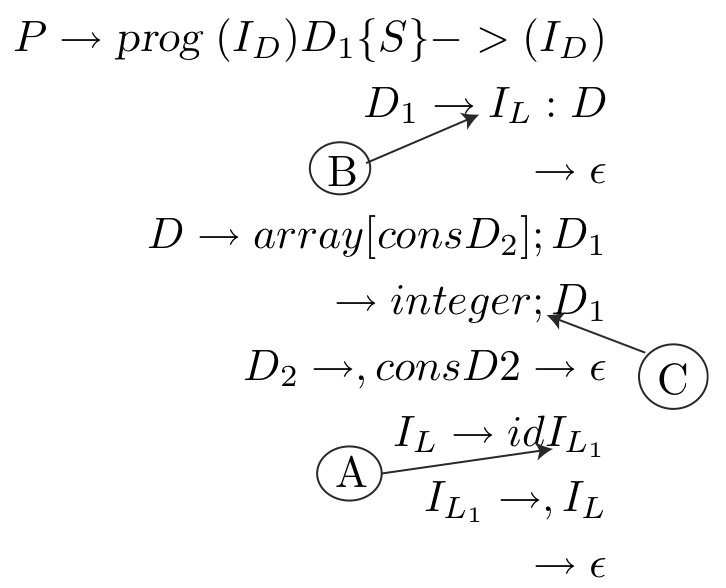
\includegraphics[width=4in]{declSemActA.png} 
   \caption{Declaration Semantics Example}
   \label{fig:example}
\end{figure}

%\subsubsection{Declarations}
Declaration statements primarily store information in the symbol table.  The entries are initiated when a symbol is first detected in the tokenizer.  The parser supplies the context of such a declaration.  Declarations may include: 
\begin{enumerate}
\item Identifiers 
\item Identifier Lists
\item Array Sub lists (indices).  
\end{enumerate}
These three types have semantic actions that are required to obtain symbol entries from the parser.  Once the parser indicates a enough information is acquired,  then that information is used to augment the symbol table.  Note that the quad table is not directly effected by a declaration statement.  

Example:
\[
\left(
\begin{array}{l}
\textbf{Production} \\
P \to \textsl{prog} (I_L ) D_1  \{ S \} \textsl{-}> (I_L) \\
\hline
D_1 \to I_L : D  \\
\to \epsilon   \\
\hline 
D \to \textsl{ array } [ \textsl{ cons }  D_2 ]; D_1   \\
\to \textsl{ integer }; D_1    \\
\hline
D_2 \to , \textsl{ cons } D_2   \\
\to \epsilon   \\
\hline
I_L \to id I_{L_1}     \\
\hline
I_{L_1} \to , I_L | \epsilon   \\
\hline
I_D \to id  I'_D   \\
\hline
I'_D \to [\textsl{ Sublist }  ]   \\
\to epsilon   \\
\end{array}
\right)
\]


\begin {algorithm}
\caption{ Semantic action $\alpha$, a.k.a. Acquire Identifier, also $\iota$ Dimension Acquisition  }
\label{alg:A0}
\begin{algorithmic}
%Arguments:  Token to pushed, NT. \\
\STATE \textrm { PUSH NT }  Token to be adjusted in the symbol table
\end{algorithmic}
\end{algorithm}

\begin {algorithm}
\caption{ Semantic action $\beta$, a.k.a. start declarations }
\label{alg:B0}
\begin{algorithmic}
%No arguments
\STATE \textrm { PUSH \# }  Push a token stopper to the stack
\end{algorithmic}
\end{algorithm}

\begin {algorithm}
\caption{ Semantic action $\gamma$, a.k.a. start array dimensions }
\label{alg:B0}
\begin{algorithmic}
%Arguments:  Token to pushed, NT.
\STATE \textrm { PUSH \# }  Push a token stopper to the stack
\STATE \textrm { PUSH NT }  Push a dimension on the stack
\end{algorithmic}
\end{algorithm}

\begin {algorithm}
\caption{ Semantic action $\eta$}
\label{alg:W2}
\begin{algorithmic}
\STATE \textrm {a := pop (SAS) }
\STATE \textrm {while $a \neq \# $ do }
\STATE \hspace {0.5 cm} \textrm { ST[a].type := integer  }
\STATE \hspace {0.5 cm} \textrm { a := pop (SAS) }
\end{algorithmic}
\end{algorithm}


\begin {algorithm}
\caption{ Semantic action $\delta$}
\label{alg:W2}
\begin{algorithmic}
\STATE \textrm {b := new vector }
\STATE \textrm {a := pop (SAS) }
\STATE \textrm {while $a \neq \# $ do }
\STATE \hspace {0.5 cm} \textrm { b.add(a)  }
\STATE \hspace {0.5 cm} \textrm { a := pop (SAS) }
\STATE \textrm {a := pop (SAS) }
\STATE \textrm {while $a \neq \# $ do }
\STATE \hspace {0.5 cm} \textrm { ST[a].type := array  }
\STATE \hspace {0.5 cm} \textrm { ST[a].dimensions := rev(b) }
\STATE \hspace {0.5 cm} \textrm { a := pop (SAS) }
\end{algorithmic}
\end{algorithm}

\begin{figure}[htbp] %  figure placement: here, top, bottom, or page
   \centering
   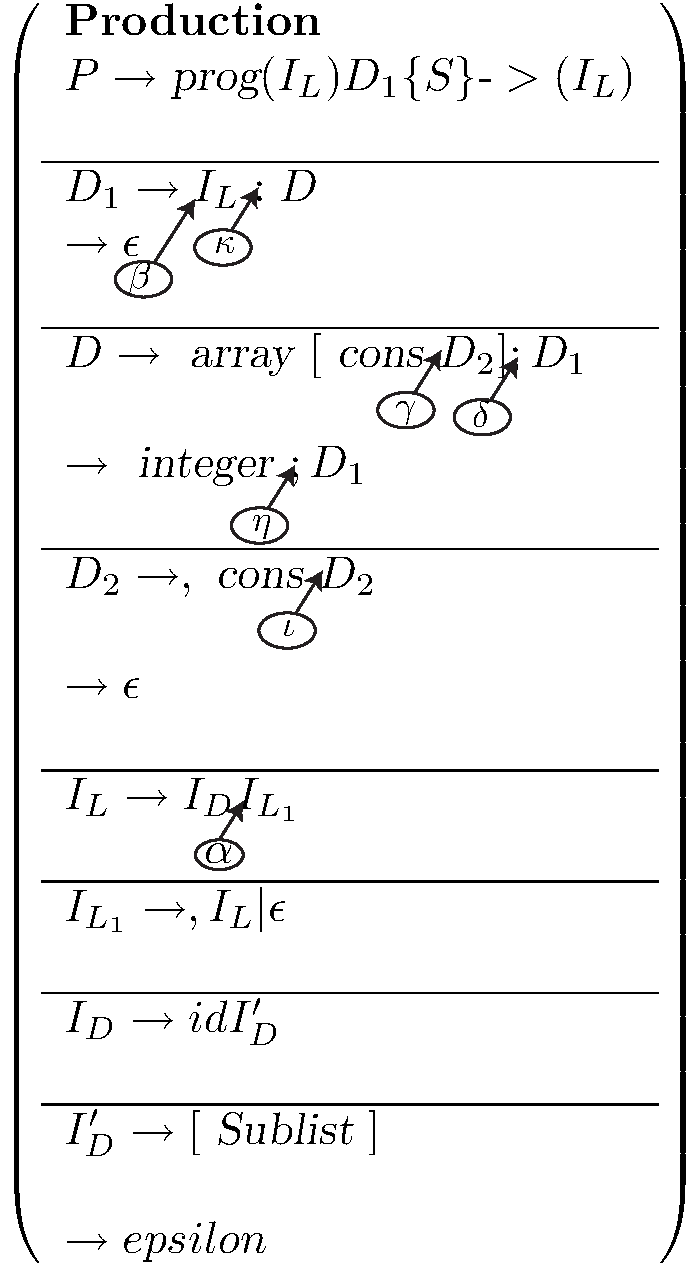
\includegraphics[width=4in]{declSemActB.pdf} 
   \caption{Declaration Semantics Example}
   \label{fig:example}
\end{figure}


\subsection {Evaluations}
Evaluation semantics:  $<$, $>$, $\le$, $\ge$, eq, neq, $+$ , $-$, $*$, $\div$, and mod  all have similar semantics:

\[ E \to \nu E_1 E_2 \]
\[ C \to \nu E_1 E_2 \]

\begin {algorithm}
\caption{ Semantic action $\alpha$ }
\label{alg:E1}
\begin{algorithmic}
\STATE \texttt { a := POP (SAS) }  Results of $E_1$
\STATE \texttt { b := POP (SAS) }  Results of $E_2$
\STATE \texttt { c := gentemp }  
\STATE \texttt { genquad ( $\nu$, b, a, c) }

\end{algorithmic}
\end{algorithm}


\subsection {Reusing Temporary Names}
What actions should occur with semantic action operation newtemp?  
\begin{enumerate}
\item The operation requests a new entry in the scope's symbol table.    
\item Also, it is with these temporary variables that optimizations can be made.  
\item Where are temporaries generated:
\begin{itemize}
\item Majority in syntax directed translation of expression.  
\item ``The lifetimes of these temporaries are nested like matching pairs of balanced parentheses.  ''    An optimization may involve modifying gentemp (newtemp) such that ``it uses a small array in a procedure's data area to hold the temporaries.''   This array is organized as a stack, and tends to be used in this fashion.  
\end{itemize}
\item ``A reasonable strategy is to create a new name whenever we create an additional definition or use for a temporary or move its computation.''   
\end{enumerate}


\newpage
\subsection  {Addressing Array Elements}
\begin{enumerate}
\item ``Elements of an array can be accessed quickly if the elements are stored in a block of consecutive locations.''  The equation is 
\[ A [i] = A_{\textsl{base}} + ( i - {\textsl{lower-bound} } ) \times \textsl{width} \]
Various means of computing this equation in the semantic actions can be performed depending on how the declaration of the array is handled.   For example, the algebraic rewrite of $A[i]$ is 
\[ A[i] = A_{\textsl{base}} - \textsl{lower-bound} \times \textsl {width} + i \times \textsl{width} \]
The first sum 
\[ C  = A_{\textsl{base}} - \textsl{lower-bound} \times \textsl {width}  \]  
\item ``Compile-time precalculation can also be applied to address calculations of elements of multi-dimensional arrays.''    This is a classic representation issue that must be addressed in most stages of language and compiler design.    It can obviously be ignored in lexical analysis.   

In most cases, it is simply a matter of define the following parameters
\begin{itemize}
\item Lower bound 
\item Fastest Variance in Subscripts
\end{itemize}
\item A more significant issue in intermediate code generation is generating references for array(s) and their indices.  
\begin{itemize}
\item Left most expression semantic action association:  \\
This idea binds the semantic actions of the array to the first index of the list as opposed to the array identifier itself.  
\item Number of dimensions and array of dimension values must be two properties of the symbol table record(s).  
\item Included in the symbol table must be location and offset of the array.  
\end{itemize}

\end{enumerate}

\subsection {Translation Scheme for Addressing Array Elements}
Diagram for the example.  






\subsection {Type Conversion within Assignment}
\begin{quote}
In practice, there would be many different types of variables and constants, so the compiler must either reject certain mixed-type operations or generate appropriate coercion (type conversion) instructions.  
\end{quote}
This issue is not in the grammar that is being presented in Cooke's class, but is common in procedural languages.  

Figure 8.19 shows the algorithm of Type Conversion for simple addition expressions.   The concept deals with converting arguments into compatible types.  Obviously, there is not always a common type between two arguments.   This issue is critical as data types are allowed to become more complex.    

The example presented by Ullman is relatively simple and present in most commonly used procedural and object oriented languages.  


\subsection {Accessing Fields in Records}
\begin{quote}
The compiler must keep track of both the types and relative addresses of the fields of a record.  An advantage of keeping this information in symbol-table entries for the field names is that the routine for looking up names in the symbol tables can also be used for field names.  
\end{quote}



Note that in all of this, words may have been stated about operations based on type.  However, indirect memory access was not one of them.  

It should be noted that procedural and logic programming have two separate concepts of the boolean or logic expressions in programming.     In procedural, the concept of logic is for controlling the flow of the program.  Although a procedural program can evaluate a set of boolean expressions to either true or false, and hence be used to evaluate a complex expression, it is not the same as a answer set or other resolution type concepts.    

This section examines the procedural component of logic evaluations.  Another section in the context of logic oriented semantics handles answer set semantics and reviews existing papers on the subject.  

\newpage
\section {Statements}


Statement semantics include some boolean and numeric evaluations as well as boolean expressions.   

\[
\left(
\begin{array}{l}
\hline 
S \to \textsl{:=} \textsl{id} E ; S   \\
\to \{ S \} S^3   \\
\to \epsilon 	\\
\hline
S' \to \textsl{ else } \{ S \} ; S   \\
\to ; S	\\
\hline
S'' \to C ; S   	\\
\to E ; S   		\\
\hline
S^3 \to \textsl{ when } C S'   \\
\hat{ } \textsl{ when } S''   \\
\end{array}
\right)
\]

\begin {algorithm}
\caption{ Semantic action $\lambda$ and $\gamma$ }
\label{alg:lambda0}
\begin{algorithmic}
\STATE \texttt {PUSH NQ}
\STATE \texttt {genquad (jmp, , , ) }
\end{algorithmic}
\end{algorithm}

\begin {algorithm}
\caption{ Semantic action $\mu$ }
\label{alg:lambda2}
\begin{algorithmic}
\STATE \texttt { a := POP (SAS) }  conditional result
\STATE \texttt { b := POP (SAS) }  end of the statement
\STATE \texttt { c := POP (SAS) }  beginning of the statement (at the jump)
\STATE \texttt { genquad ( jtrue, a, , c + 1) }
\STATE \texttt { QUADS [c,4] := b+ 1 }
\STATE \texttt { QUADS [b,4] := NQ }
\end{algorithmic}
\end{algorithm}

\begin {algorithm}
\caption{ Semantic action $\eta$ }
\label{alg:lambda3}
\begin{algorithmic}
\STATE \texttt { a := POP (SAS) }  conditional result
\STATE \texttt { b := POP (SAS) }  end of the statement
\STATE \texttt { c := POP (SAS) }  beginning of the statement (at the jump)
\STATE \texttt { genquad ( jtrue, a, , c + 1) }
\STATE \texttt { QUADS [c,4] := b+ 1 }
\STATE \texttt { PUSH b}
\end{algorithmic}
\end{algorithm}

\begin {algorithm}
\caption{ Semantic action $\chi$ }
\label{alg:lambda3}
\begin{algorithmic}
\STATE \texttt { b :=  POP }
\STATE \texttt { QUADS [b,4] := NQ }
\end{algorithmic}
\end{algorithm}

\begin {algorithm}
\caption{ Semantic action $\iota$ }
\label{alg:lambda3}
\begin{algorithmic}
\STATE \texttt { c := POP } Results of Conditional
\STATE \texttt { b := POP } Jump coordinates after statement
\STATE \texttt { a := POP } Jump coordinates before statement
\STATE \texttt { QUADS [a,4] := b + 1 }
\STATE \texttt { QUADS [b,4] := b + 1 }
\STATE \texttt { genquad (jtrue, c, , a + 1 )  }
\end{algorithmic}
\end{algorithm}

\begin {algorithm}
\caption{ Semantic action $\kappa$ }
\label{alg:lambda3}
\begin{algorithmic}
\STATE \texttt { c := POP } Results of Expression
\STATE \texttt { b := POP } Jump coordinates after statement
\STATE \texttt { a := POP } Jump coordinates before statement
\STATE \texttt { genquad ( jmp, , , a + 1 ) }   Jump to the statement
\STATE \texttt { d := NQ }  Location of the test
\STATE \texttt { genquad ( - , c, 1, c ) }   decrement the count
\STATE \texttt { e := gentemp }
\STATE \texttt { genquad ( $\le$, c , 0, e ) } 
\STATE \texttt { genquad (jtrue, e, , a + 1 )  }
\STATE \texttt { QUADS [a,4] := b + 1 }
\STATE \texttt { QUADS [b,4] := d  }
\end{algorithmic}
\end{algorithm}

\begin {algorithm}
\caption{ Semantic action $\beta$ }
\label{alg:lambda0}
\begin{algorithmic}
\STATE \texttt {b := pop}
\STATE \texttt {a := id }
\STATE \texttt {genquad (:= , b, , a ) }
\end{algorithmic}
\end{algorithm}

\begin{figure}[htbp] %  figure placement: here, top, bottom, or page
   \centering
   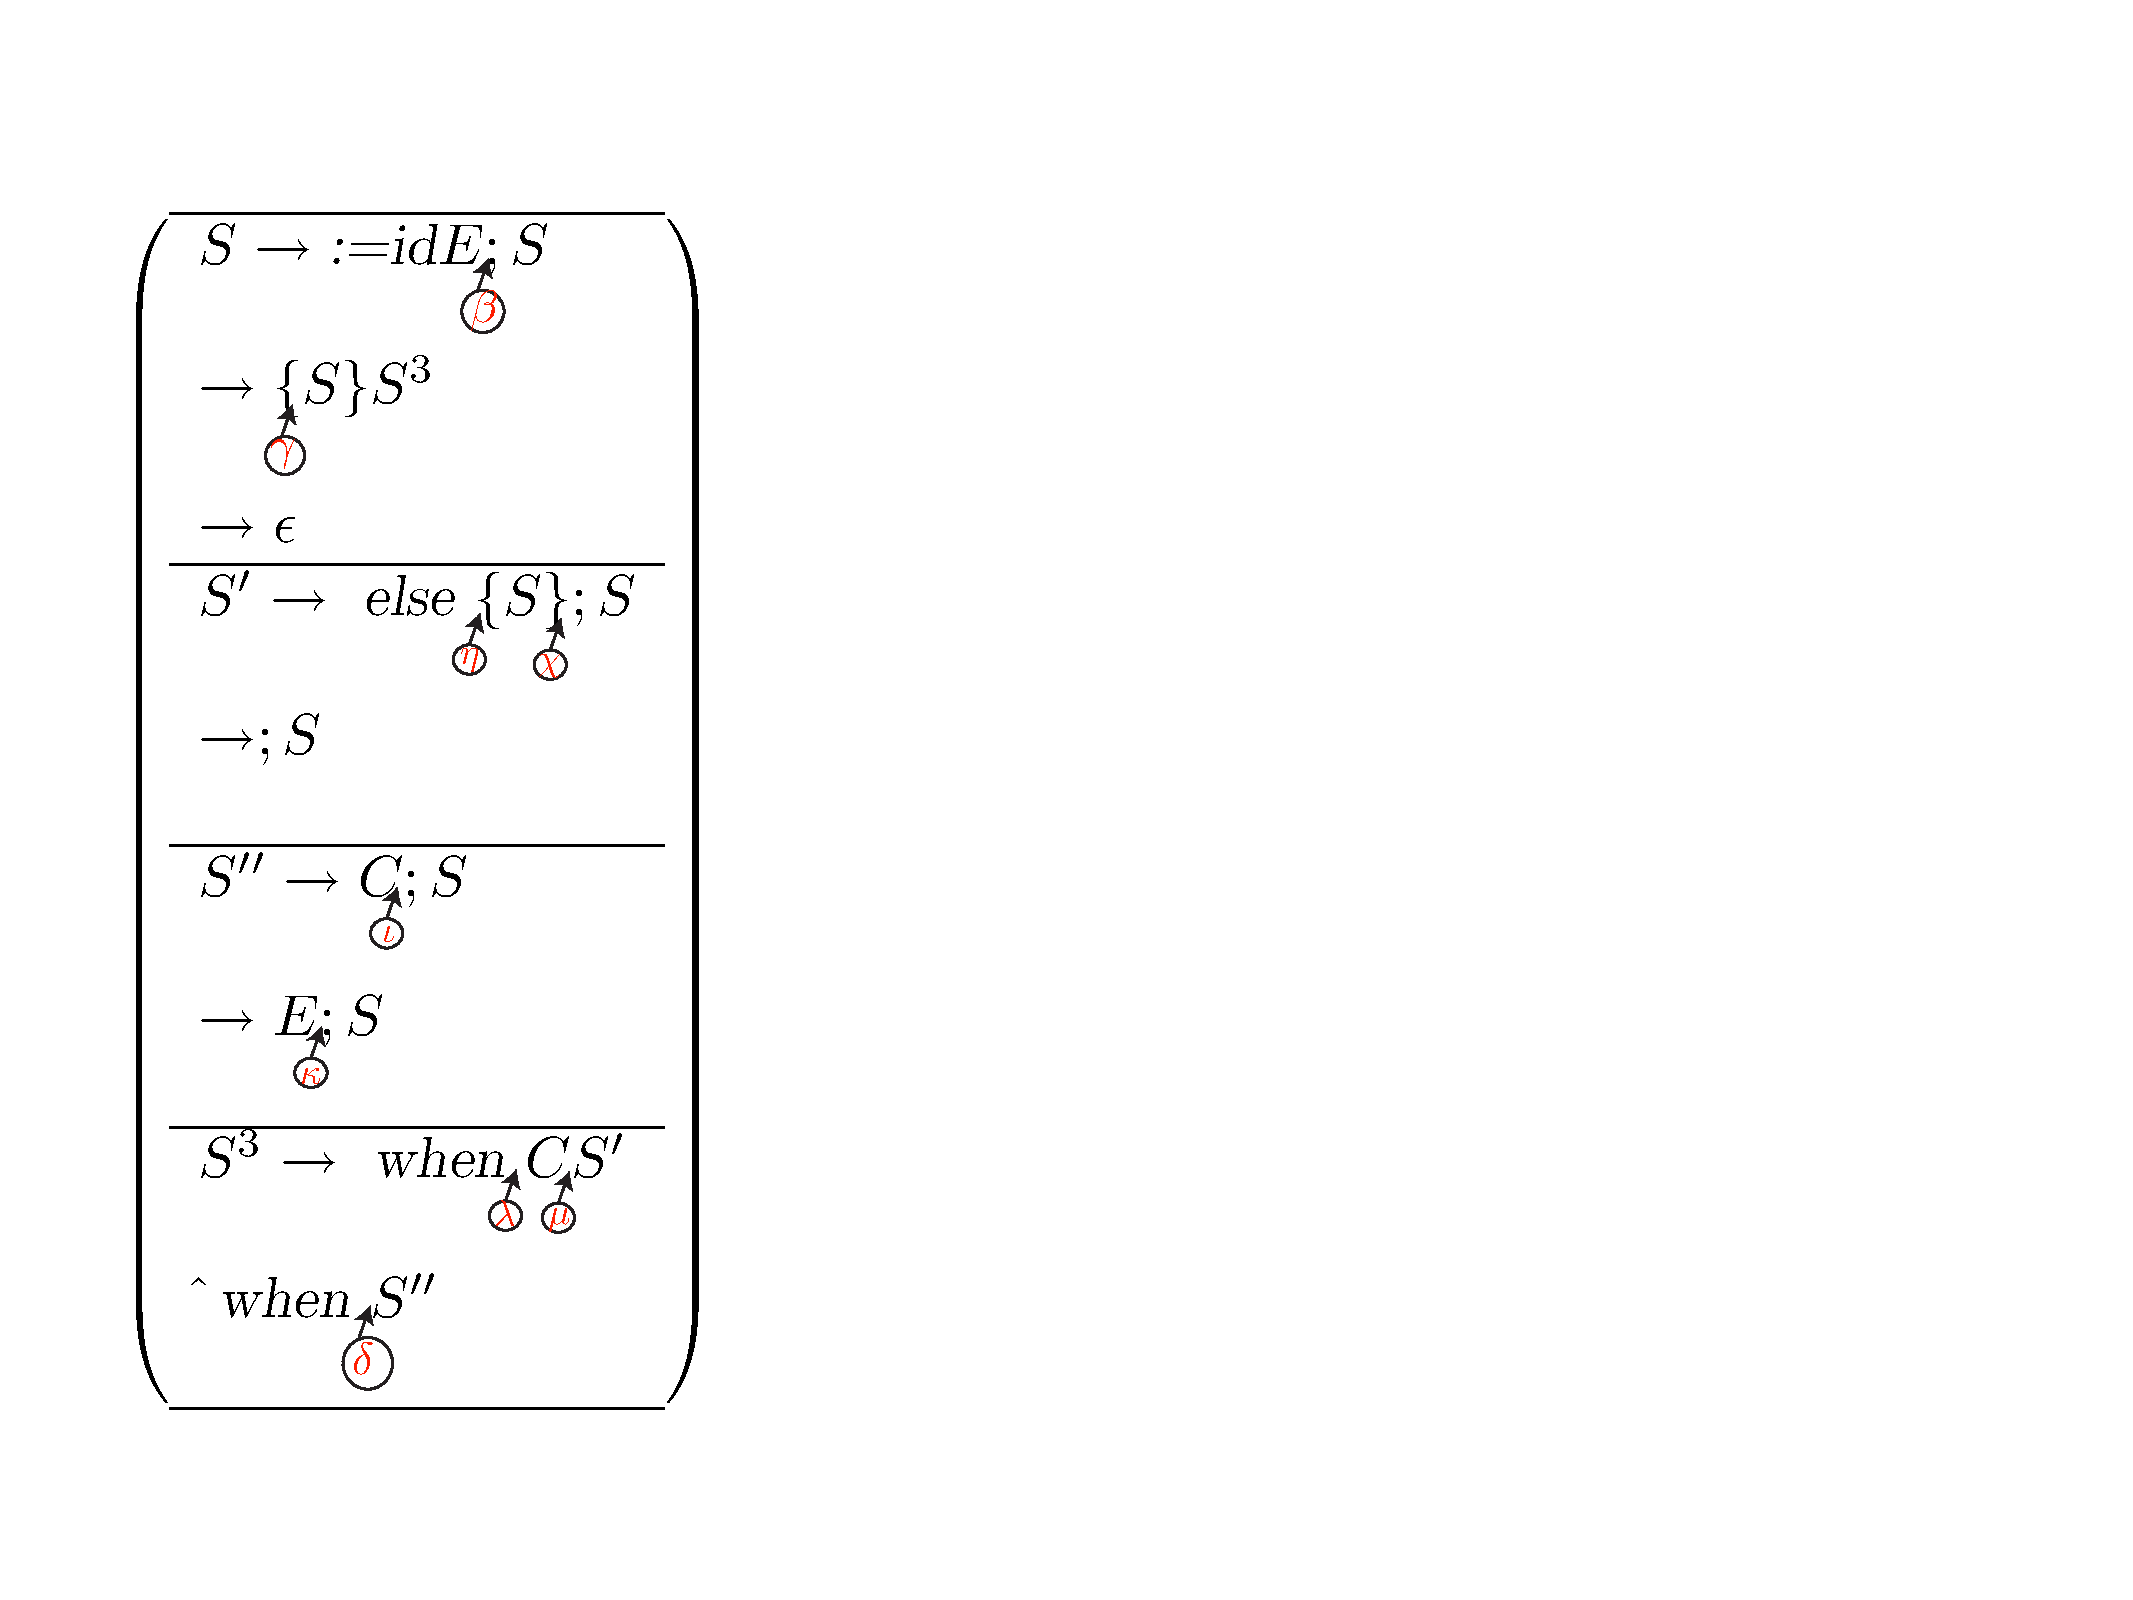
\includegraphics[width=2in]{statementsA.pdf} 
   \caption{Statements Semantic Actions}
   \label{fig:example}
\end{figure}

\begin{figure}[htbp] %  figure placement: here, top, bottom, or page
   \centering
   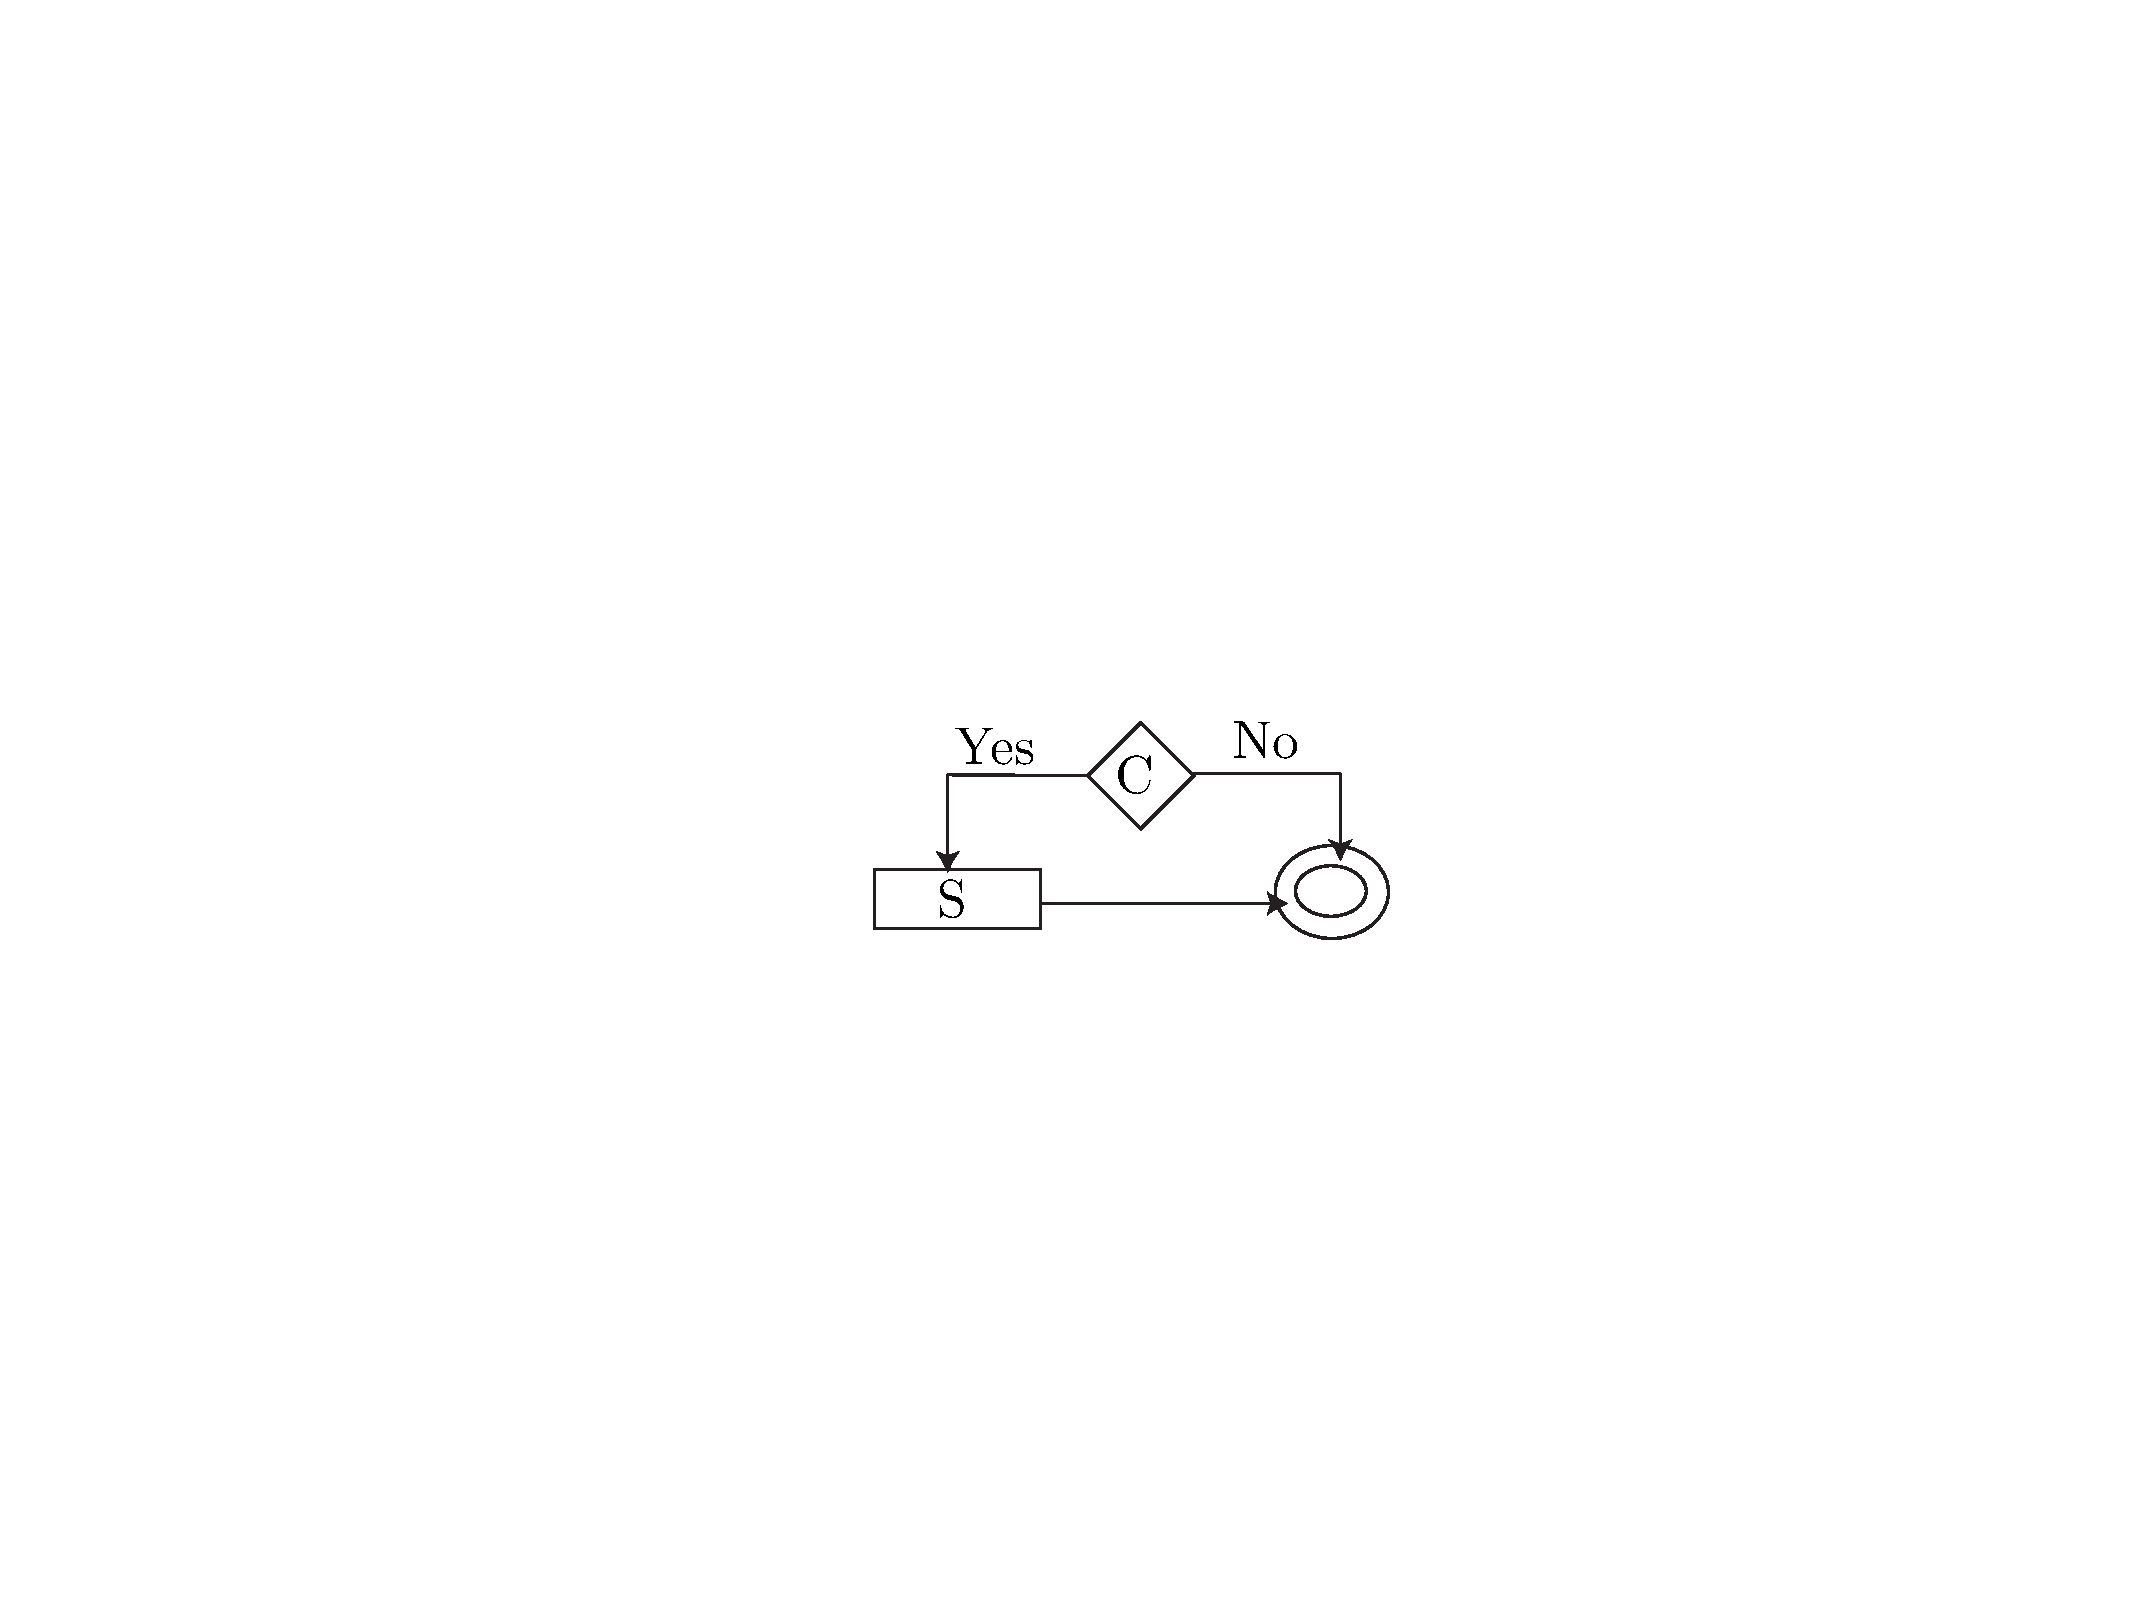
\includegraphics[width=2in]{statementWhenC.pdf} 
   \caption{When Condition Semantic Actions}
   \label{fig:example}
\end{figure}

\begin{figure}[htbp] %  figure placement: here, top, bottom, or page
   \centering
   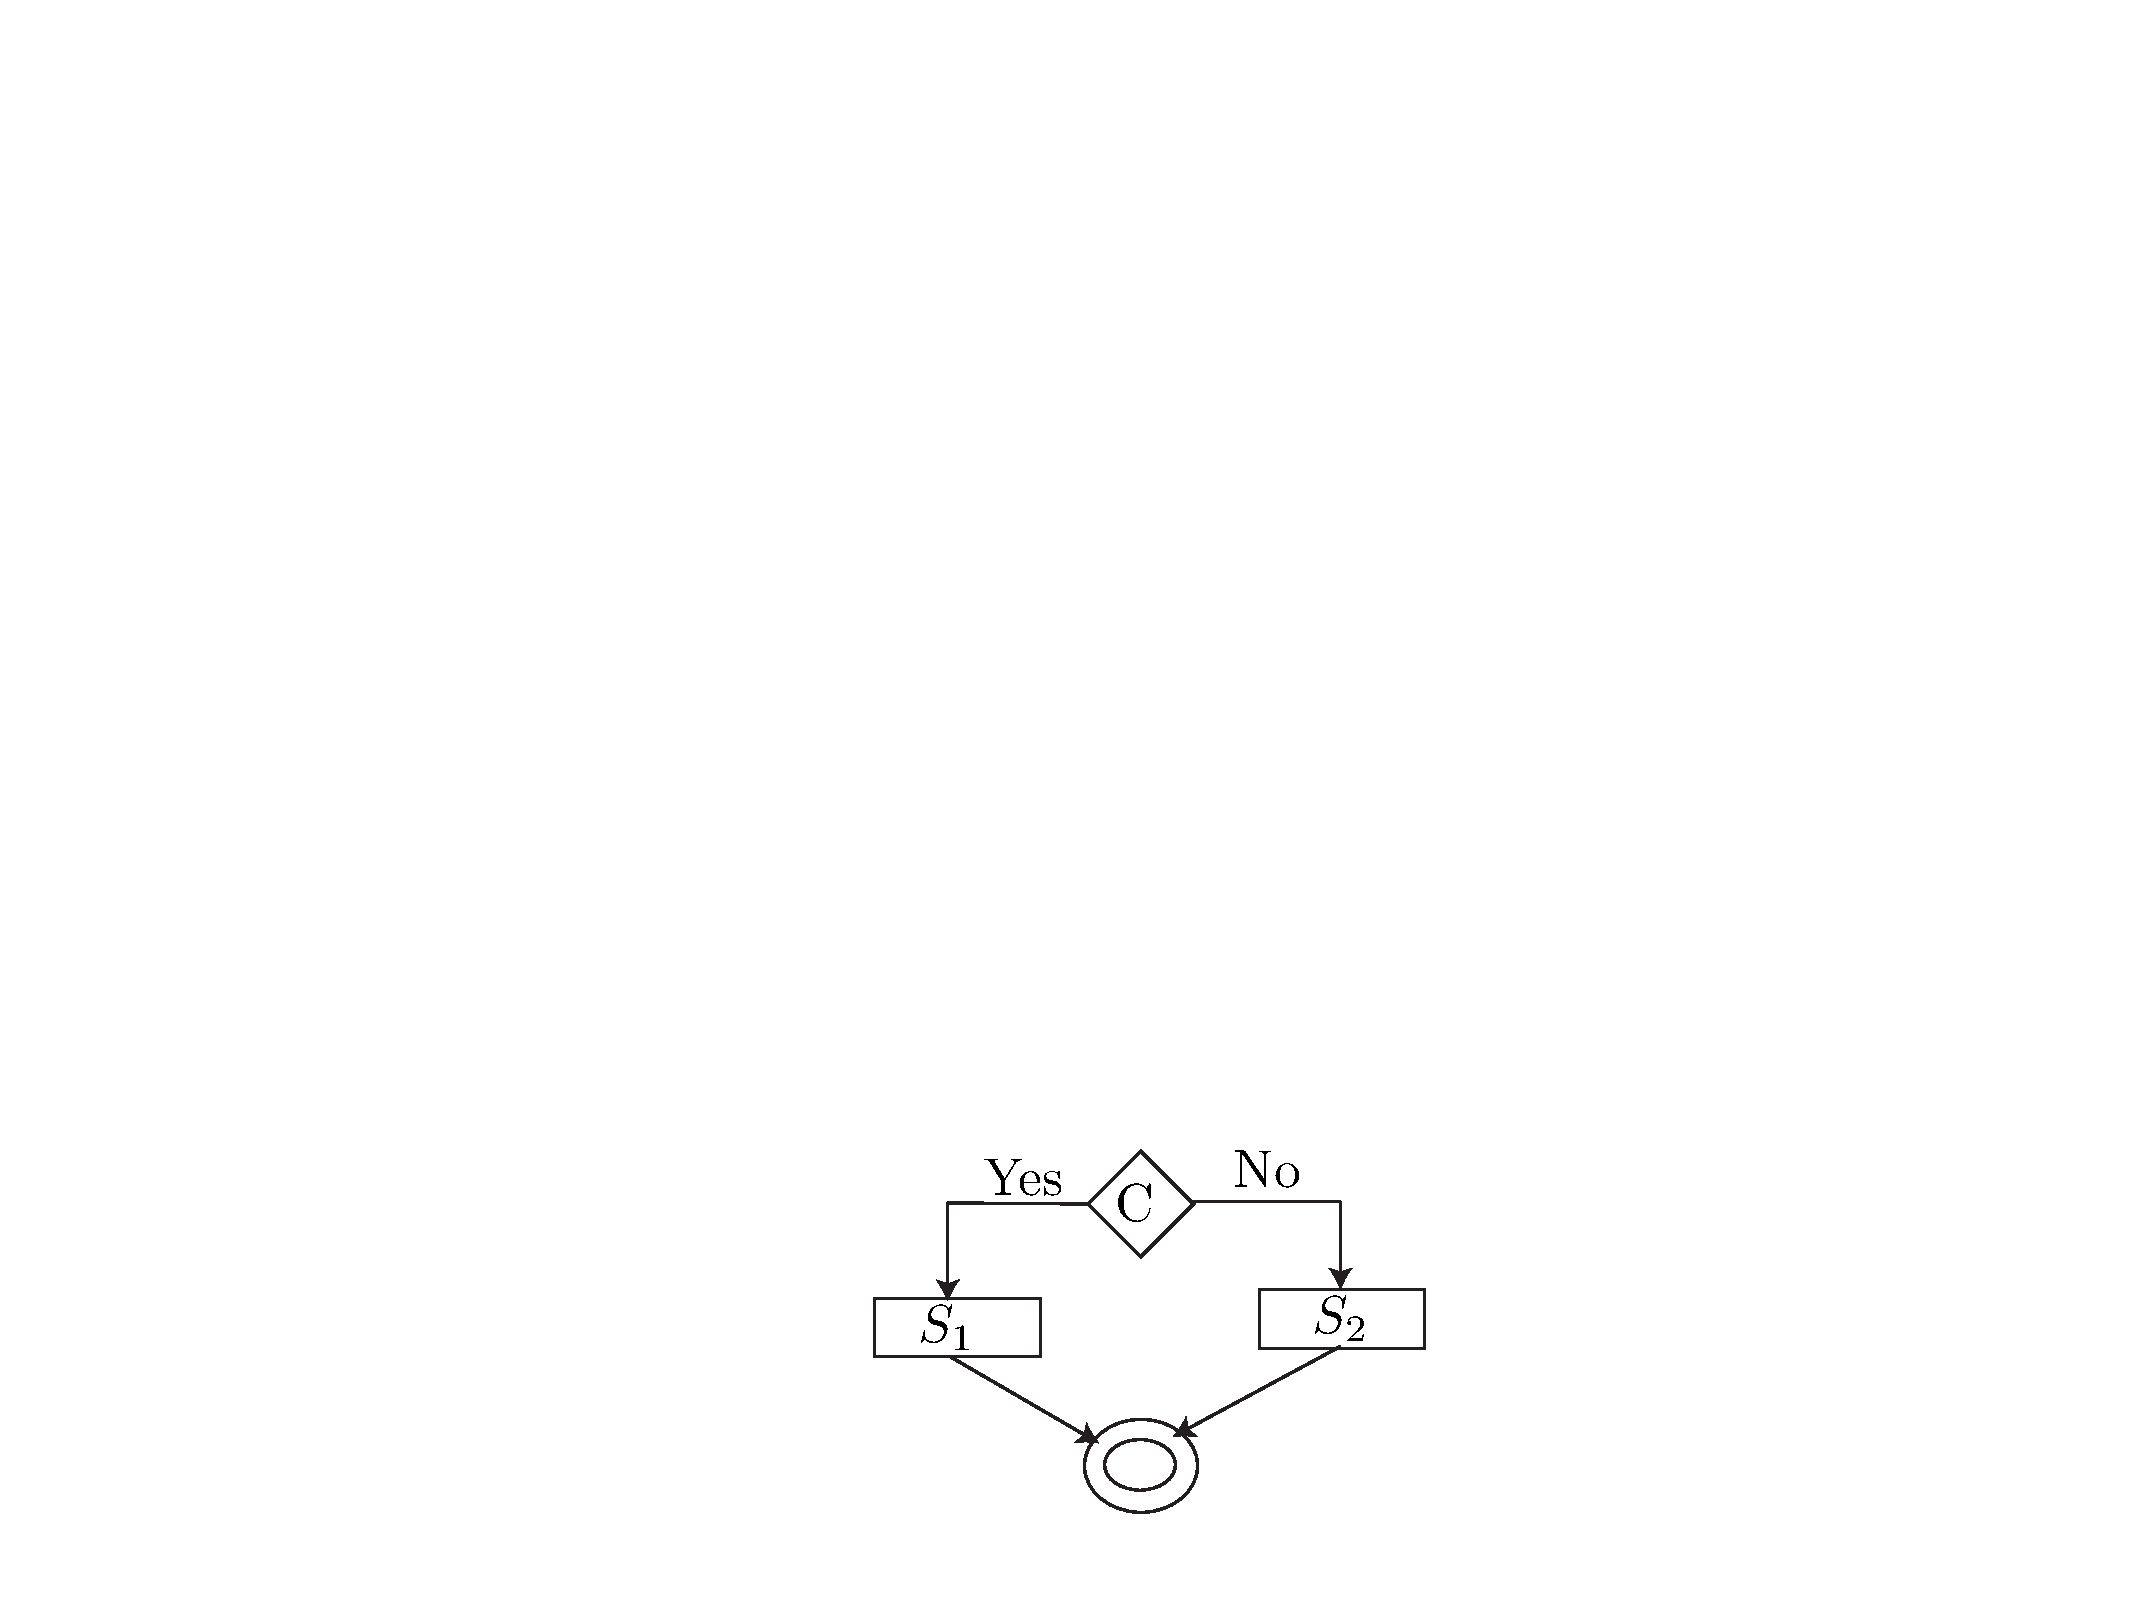
\includegraphics[width=2in]{statementWhenElse.pdf} 
   \caption{When Condition Else Semantic Actions}
   \label{fig:example}
\end{figure}

\begin{figure}[htbp] %  figure placement: here, top, bottom, or page
   \centering
   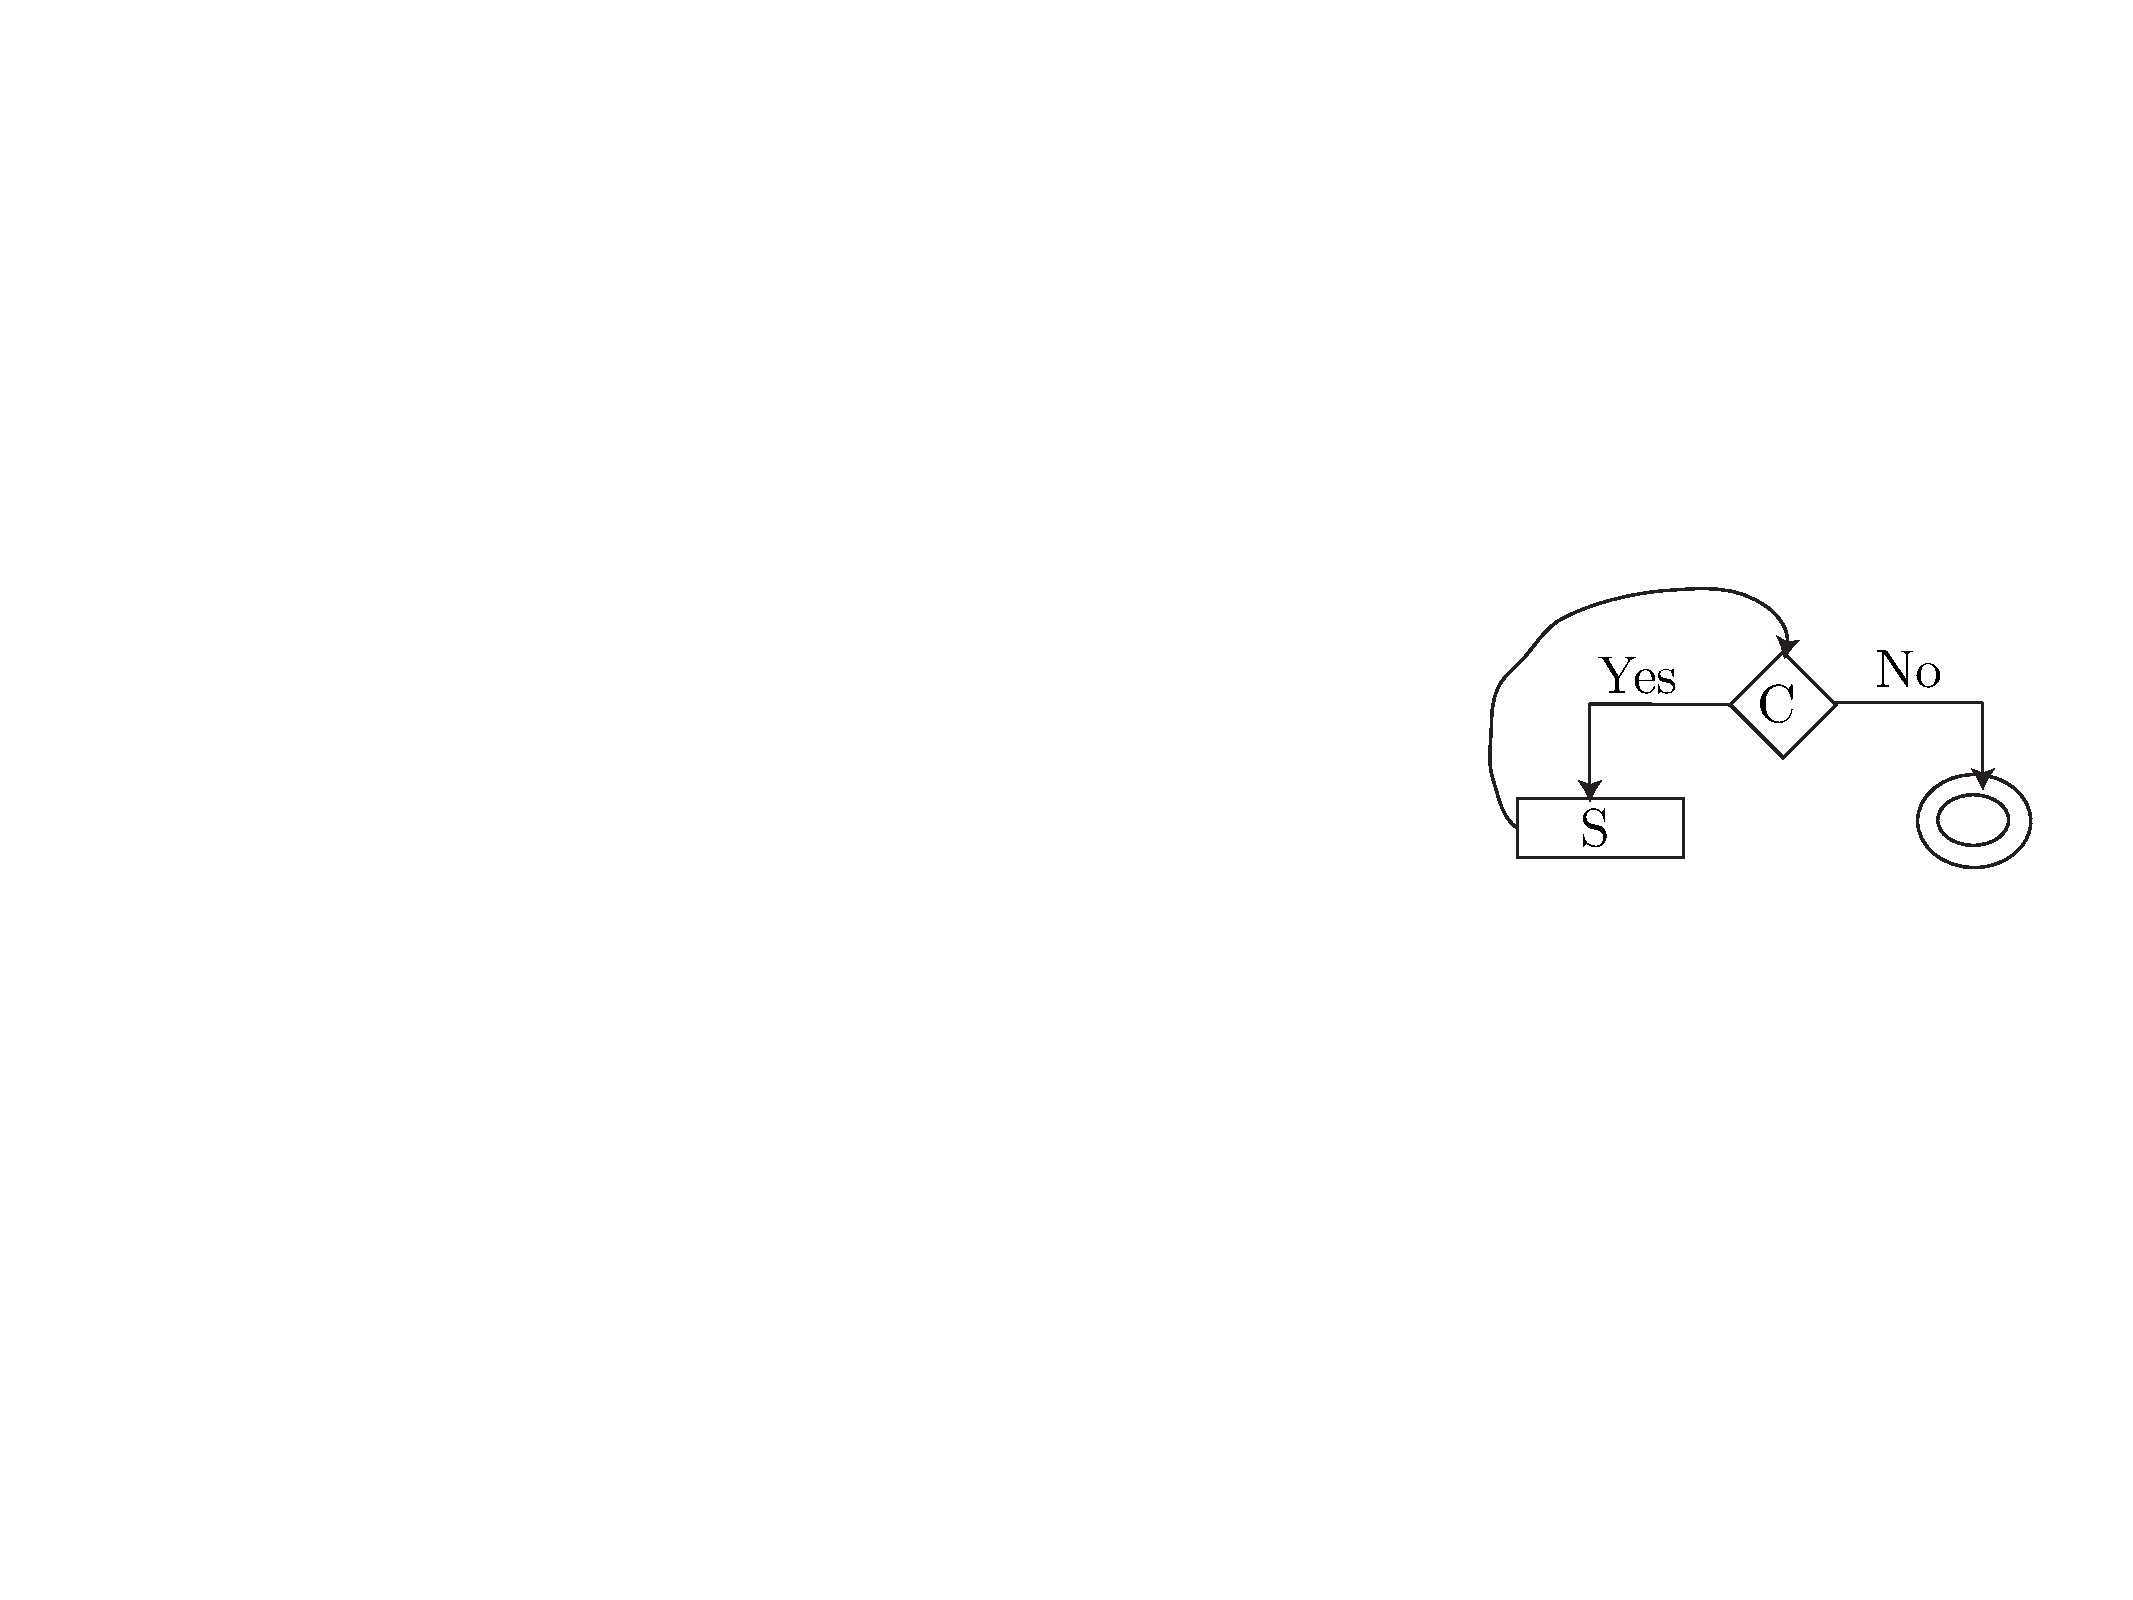
\includegraphics[width=2in]{statementCarrotC.pdf} 
   \caption{Carrot Condition Semantic Actions, a.k.a. a while loop}
   \label{fig:example}
\end{figure}


\begin{figure}[htbp] %  figure placement: here, top, bottom, or page
   \centering
   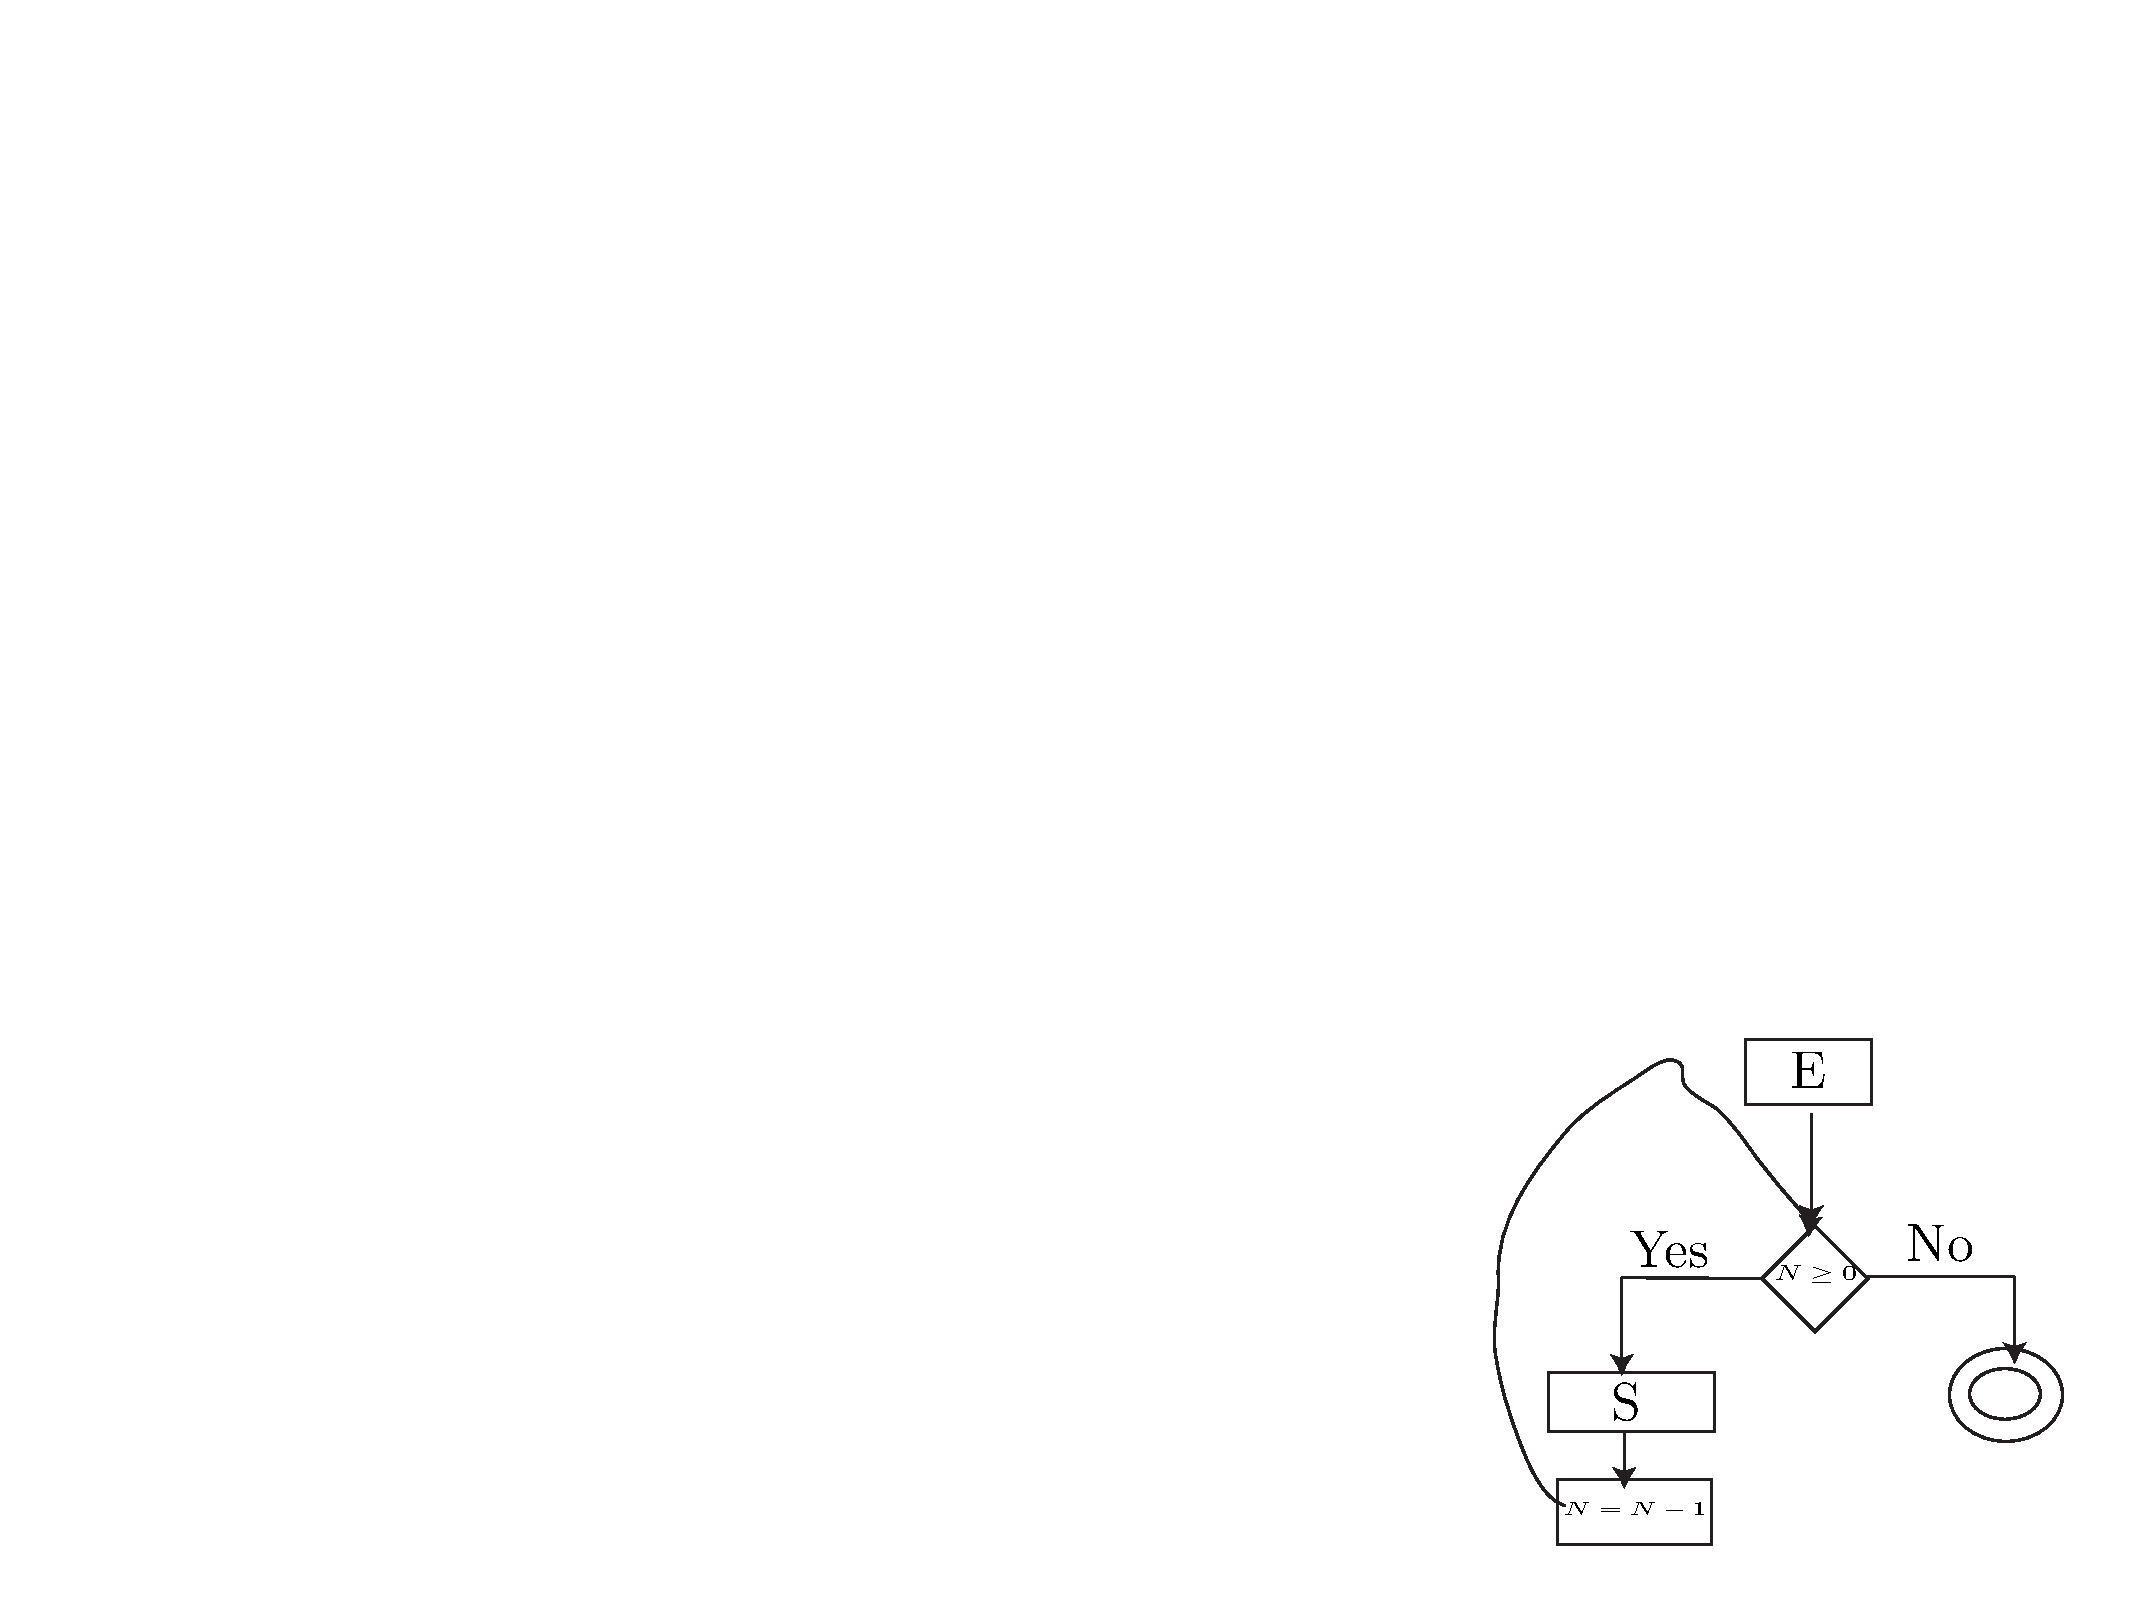
\includegraphics[width=2in]{statementCarrotE.pdf} 
   \caption{Carrot Expression Semantic Actions, a.k.a. a for loop}
   \label{fig:example}
\end{figure}

\newpage
\subsection {Methods of Translating Boolean Expressions} 

\begin{enumerate}
\item Principle means of encoding boolean expressions
\begin{enumerate}
\item Represent the states of boolean expressions numerically \\
\begin{enumerate}
\item Operations become a form of boolean mathematics which inherent to the intermediate machine.  
\item The logical operators $\wedge$, $\vee$ and $\neg$ (and, or, and not) can be represented by branching statements.  
\item The logical operators can also be represented as actual quad operations.  
\end{enumerate}

\item   Flow control representation:  The method identify the boolean state by position in the program.  
\end{enumerate}
\item Optimizations in the flow control and numerical evaluation can be made in cases where by the outcome is determined with out evaluating the full condition.  
\end{enumerate}


\subsubsection{Example: Conditionals}
\[
\left(
\begin{array}{l}
\to \textsl{ and } C \textsl{ } C 	  \\
\to \textsl{ or } C \textsl{ } C   \\
\to \textsl{ not } E    \\
\end{array}
\right)
\]
There is a brute force method for handling conditionals such as these.    Three semantic actions are necessary for this prefix example.    The general flow is the same for other notations, but this notation provides a very simple set of actions.  

\begin {algorithm}
\caption{ Semantic action $\beta$, a.k.a. the ``And''  action }
\label{alg:andaction}
\begin{algorithmic}
\STATE \texttt {a := pop}  $C_2$ result
\STATE \texttt {b := pop}  $C_1$ result
\STATE \texttt {c := NQ }  First quad operation
\STATE \texttt {d := gentemp}  Result of this conditional
\STATE \texttt {genquad (jfalse, b, , , ) }  
\STATE \texttt {genquad (jfalse, a, , , ) }  
\STATE \texttt {genquad (:=, d, , , true ) }  
\STATE \texttt {genquad (jmp, , , , ) }  
\STATE \texttt {genquad (:=, d, , , false ) }  
\STATE \texttt {QUADS[c].results := c + 4 }  
\STATE \texttt {QUADS[c+1].results := c + 4 }  
\STATE \texttt {QUADS[c + 3].results := c + 5 }  
\end{algorithmic}
\end{algorithm}


\begin {algorithm}
\caption{ Semantic action $\gamma$, a.k.a. the ``or''  action }
\label{alg:andaction}
\begin{algorithmic}
\STATE \texttt {a := pop}  $C_2$ result
\STATE \texttt {b := pop}  $C_1$ result
\STATE \texttt {c := NQ }  First quad operation
\STATE \texttt {d := gentemp}  Result of this conditional
\STATE \texttt {genquad (jtrue, b, , , ) }  
\STATE \texttt {genquad (jtrue, a, , , ) }  
\STATE \texttt {genquad (:=, d, , , false ) }  
\STATE \texttt {genquad (jmp, , , , ) }  
\STATE \texttt {genquad (:=, d, , , true ) }  
\STATE \texttt {QUADS[c].results := c + 4 }  
\STATE \texttt {QUADS[c+1].results := c + 4 }  
\STATE \texttt {QUADS[c + 3].results := c + 5 }  
\end{algorithmic}
\end{algorithm}


\begin {algorithm}
\caption{ Semantic action $\eta$, a.k.a. the `not''  action }
\label{alg:andaction}
\begin{algorithmic}
\STATE \texttt {a := pop}  $C_1$ result
\STATE \texttt {c := NQ }  First quad operation
\STATE \texttt {d := gentemp}  Result of this conditional
\STATE \texttt {genquad (jtrue, a, , , ) }  
\STATE \texttt {genquad (:=, d, , , true ) }  
\STATE \texttt {genquad (jmp, , , , ) }  
\STATE \texttt {genquad (:=, d, , , false ) }  
\STATE \texttt {QUADS[c].results := c + 3 }  
\STATE \texttt {QUADS[c+1].results := c + 3 }  
\STATE \texttt {QUADS[c + 2].results := c + 4 }  
\end{algorithmic}
\end{algorithm}

\begin{figure}[htbp] %  figure placement: here, top, bottom, or page
   \centering
   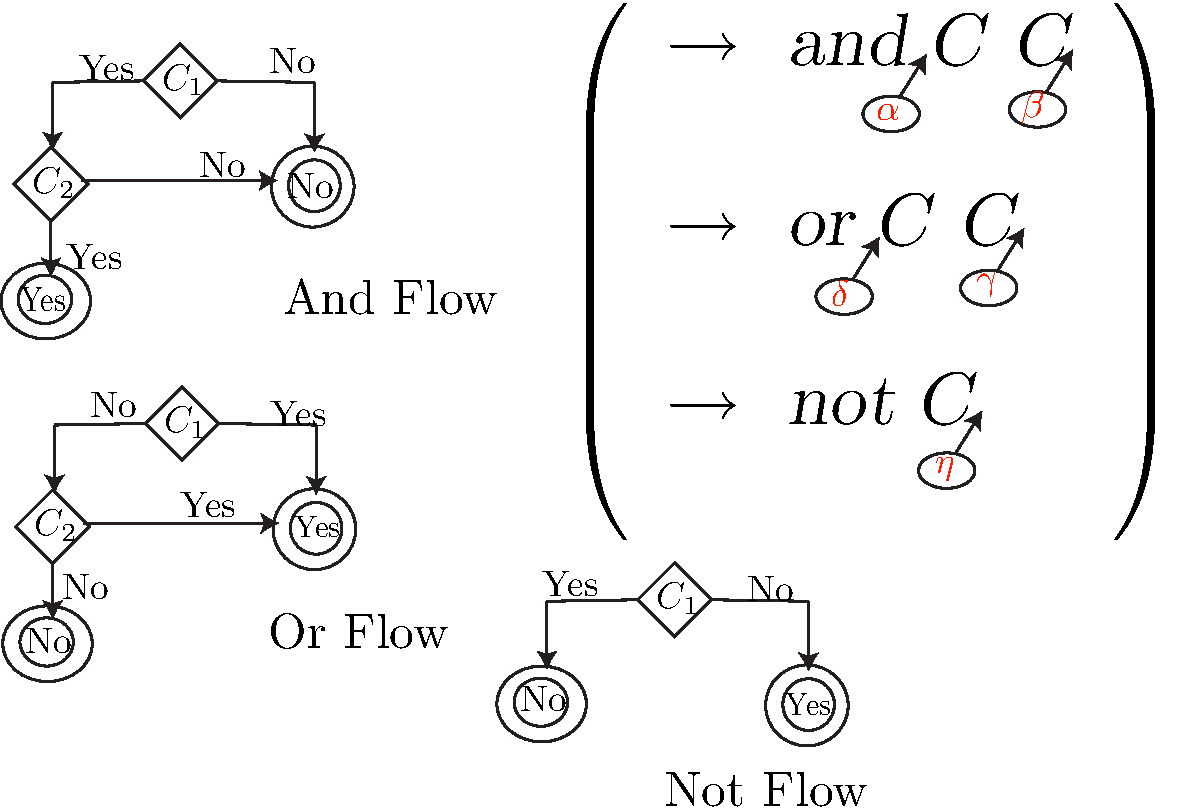
\includegraphics[width=4in]{statementConditional.pdf} 
   \caption{Conditional Statement}
   \label{fig:example}
\end{figure}

\subsection {Flow Control Statements}  
The three basic procedural control constructs:
\begin{enumerate}
\item if - then
\item if - then - else
\item while - do
\end{enumerate}
In each of these cases, there is a conditional production part of these flow control statements which is evaluated true or false, and any branching can be based those two conditions.  

\subsection{Mixed-Mode Boolean Expresion}

A semantic to be considered in procedural programming is 
\[  ( a < b) + (b < a) \]  
In this case, it is an arithmetic expression.    Not all procedural syntax allows this sort of mixing.   
\begin{enumerate}
\item Conditionals are special types of expressions.
\item The case of mixed expressions forces conditional expressions include type information.   Reference Figure 8.25.  
\end{enumerate}


\section {Case Statements}
\begin{quote}
There is a selector expression which is to evaluated, followed by $n$ constant values that the expression might take, perhaps including a default ``value,'' which always matches the expression if no other value does.  The intended translation of a switch is code to:
\begin{enumerate}
\item Evaluate the expression.
\item Find which value in the list of cases is the same as the value of the expression.  Recall that the default value matches the expression if non of the values explicitly mentioned in case does.  
\item Execute the statement associated with the value found.   
\end{enumerate}
\end{quote}

Two methods exist for implementing such a construct.  One is to use a series of branch statements.  The other is to use a lookup table consisting of pairs (value and code location pairs).    This becomes a symbol table problem for efficiency.  

Reference Figures 8.27 and 8.28  .  

\begin{quote}
We process each statement \textbf{case} $V_1$: $S_i$ by emitting the newly created created label $L_i$, followed by the code for $S_i$, followed by the jump \textsl{goto next}.  Then when when the keyword \textbf{end} terminating the body of the switch is found, we are ready to generate the code for the n-way branch.  Reading the pointer-value pairs on the case stack from the bottom to the top, we can generate a sequence of three-address statements of the form.
\begin{lstlisting}
case V1, L1
case V2 L2
...
case Vn Ln-1
case t  Ln
label next
\end{lstlisting}
\end{quote}

\newpage
\section {Backpatching}
\begin {quote}
The main problem with generating code for boolean expressions and flow-of-control statements in a single pass is that during one single pass we may not know the labels that control must go to at the time jump statements are generated.  
\end{quote}

\begin{quote}
Labels will be indices into this array.  To manipulate lists of labels, we use three functions:
\begin{enumerate}
\item Makelist (i)
\item Merge  (p1, p2) 
\item backpatch (p,i)
\end{enumerate}

\end{quote}


``Synthesized attributes truelist and falselist of nonterminal $E$ are used to generate jumping code for boolean expressions. ... These incomplete jumps are placed on lists pointed to by E.truelist and E.falselist, as appropriate.''  A relational operation conditional tends to have at least two jumps: the conditional jump and the unconditional jump.  Typically, the truelist belongs to the code pointed to by the  conditional jump, and the false list is associated with the code following the unconditional jump.    

Other productions end up getting fill-in values for their quad-labels by the backtrack operations.  This is due to the fact some operations fall within the statements such that they are part of branched code.    Each of these productions maintain ``a list of all conditional and unconditional jumps to the quadruple following the statement $S$ in execution order.''       

%S.begin, 
%S.nextlist, and 
%E.true mark the beginning of 
Flow control statements also include markers to indicate the start of productions nested within.    The markers are updated by any backpatch.  Another example semantic actions are prepared on Ullman's page 505.    It introduces a semantic action to assign a nextlist with the following quad.  



\end{document}   